\documentclass[zad,zawodnik,utf8]{sinol}

\usepackage{hyphenat}
\usepackage{ulem}
\usepackage{tikz}

\title{Płytkafelki}
\id{pyk}
\RAM{64}
\date{2019-03-02}
\konkurs{PreMOI}

\signature{Kubin}
\author{Jakub Bachurski}

\begin{document}
\begin{tasktext}%
\par Pewnego pięknego dnia, don Bajton uznał, że chce upiększyć drogę przed jego rezydencją. Zadecydował, że wyłoży ją \sout{płytkami} kafelkami. Wybrał też sposób, w jaki ukafelkuje drogę: weźmie dwa różne rodzaje kafelków (spośród pewnych $n$, które ma pod ręką -- można przyjąć, że ma nieskończenie wiele kafelków każdego rodzaju), i utworzy z nich dwie sąsiednie i przylegające do siebie ścieżki tej samej długości. Obie te ścieżki mają się składać z innego rodzaju kafelków. Kafelki są kwadratowe i charakteryzują się wielkością boku, która zawsze jest całkowita. Przykładowe ścieżki wyglądają tak:
\begin{center}
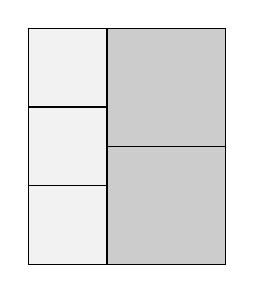
\begin{tikzpicture}
\draw[fill=gray!40, draw=black] (1, 0) rectangle (2.5, 1.5);
\draw[fill=gray!40, draw=black] (1, 1.5) rectangle (2.5, 3);
\draw[fill=gray!10, draw=black] (0, 0) rectangle (1, 1);
\draw[fill=gray!10, draw=black] (0, 1) rectangle (1, 2);
\draw[fill=gray!10, draw=black] (0, 2) rectangle (1, 3);
\end{tikzpicture}
\ \ \ \ \
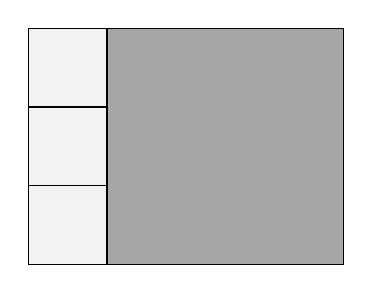
\begin{tikzpicture}
\draw[fill=gray!70, draw=black] (1, 0) rectangle (4, 3);
\draw[fill=gray!10, draw=black] (0, 0) rectangle (1, 1);
\draw[fill=gray!10, draw=black] (0, 1) rectangle (1, 2);
\draw[fill=gray!10, draw=black] (0, 2) rectangle (1, 3);
\end{tikzpicture}
\end{center}

\par Ścieżka z lewej powstała z kafelków wielkości 2 (jasne) i 3 (ciemne), a ścieżka z prawej z 2 i 6 (ciemniejsze). Obie ścieżki są długości 6.

\par Don Bajton chce, aby otrzymana ścieżka była jak najpiękniejsza. Piękno ścieżki złożonej z kafelków $a$ oraz $b$ o długości $s$ według Bajtona jest zdefiniowana w ten sposób:
\[ p = \frac{ab}{s}  \]
Jak powiedział, \textit{,,Jest już za stary na te rachunki...''}, i sam sobie nie poradzi z problemem. Czy pomożesz mu w znalezieniu pary kafelków, która daje jak najpiękniejszą ścieżkę?

\section{Wejście}
\par W pierwszej linii wejścia znajdzie się jedna liczba całkowita $n$ $(2 \le n \le 5 \cdot 10^5)$, oznaczającą ilość dostępnych don Bajtonowi rodzajów kafelków. W kolejnym wierszu jest $n$ liczb całkowitych $a_i$ $(1 \le a_i \le 10^6)$, oznaczających, że don Bajton ma kafelki o boku $a_i$. Możliwe, że liczby $a_i$ się powtórzą -- w takim wypadku są traktowane jak odmienne rodzaje o tej samej wielkości. W szczególności, tworzą ścieżkę o długości $a_i$.

\section{Wyjście}
\par Na pierwszą linię wyjścia należy wypisać $p$, a na drugą $i$ oraz $j$. $i$ oraz $j$ powinny oznaczać indeksy rodzajów kafelków, które należy wykorzystać, aby powstała ścieżka była jak najpiękniejsza. $p$ ma być równe piękności otrzymanej ścieżki. Jeżeli istnieje wiele kombinacji kafelków, które mają taką samą (maksymalną) wartość $p$, należy wybrać to z najmniejszym $i$. Jeżeli nadal istnieje wiele rozwiązań, wybierz to z najmniejszym $j$.

\pagebreak
\section{Przykłady}
\makeexamplef{in/0a.in}{out/0a.out}
\makeexamplef{in/0b.in}{out/0b.out}
\end{tasktext}
\subsection{Wyjaśnienie przykładu}
\par W pierwszym przykładzie należy wybrać kafelki wielkości 4 oraz 6. Ścieżka ułożona z tych kafelków jest długości 12, więc jej piękno to $\frac{4 \cdot 6}{12} = 2$.
\par W drugim teście przykładowym optymalnym wyborem są kafelki 15 i 30.
\end{document}